%---------------------------------------------------------------------
%
%                          analyses.tex
%
%---------------------------------------------------------------------
%
% analyses.tex
% Copyright 2015 Dr. Francisco J. Pulido
%
% This presentation belongs to the PhD titled "New Techniques and Algorithms for Multiobjective and Lexicographic Goal-Based Shortest Path Problems", distributed under the Creative Commons Licence Attribution-NonCommercial-NoDerivs 3.0, available in http://creativecommons.org/licenses/by-nc-nd/3.0/. The complete PhD dissertation is freely accessible from http://www.lcc.uma.es/~francis/

\section{Empirical analyses}
%%%%%%%%%%%%%%%%%%%%%%%%%%%%%%%%%%%%%%%%%%%%%%%%%%%%%%%%%%%%%%%%%%%%%%%%%%%%%%%%%%%%%%%%%%%%%%%%%%%%%%%%%
\begin{frame} 
\frametitle{Empirical analyses}
\Large
	\begin{itemize}
		\item Are these new algorithms \textcolor{ao}{effective}?
		\vspace{3mm}
		\item Will \lexgo \ become faster when goals get \textcolor{ao}{more restrictive}?
		\vspace{3mm}
		\item Have we achieved \textcolor{ao}{improvements over \namoa}? \\ 
		To what extent? Why?
	\end{itemize}
\end{frame}
%%%%%%%%%%%%%%%%%%%%%%%%%%%%%%%%%%%%%%%%%%%%%%%%%%%%%%%%%%%%%%%%%%%%%%%%%%%%%%%%%%%%%%%%%%%%%%%%%%%%%%%%%
\begin{frame} 
\frametitle{Empirical analyses}
\begin{columns}[onlytextwidth, t]
\column{0.5\linewidth}
	\textbf{Random grids}
	\begin{itemize}
		\item 100 $\times$ 100
		\item \textcolor{ao}{Solution depth from 20 to 100}
		\item Random costs in range [1,10]
	\end{itemize}
	\vspace{2mm}
	\begin{figure}
    	\centering
		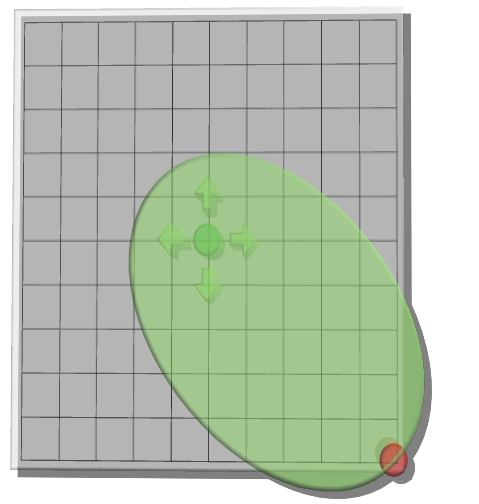
\includegraphics[scale=0.18]{figs/grids}
	\end{figure}
\column{0.5\linewidth}
	\textbf{Realistic Road maps}
	\begin{itemize}
		\item 20 random problems over \\ New York City \& Vermont State from 9th DIMACS Challenge
		\item \textcolor{ao}{Three} integer costs
		\begin{itemize}
			\item Distance 
			\item Travel time
			\item Economic cost
		\end{itemize}
	\end{itemize}
	\vspace{-5mm}
	\begin{figure}
    	\centering
		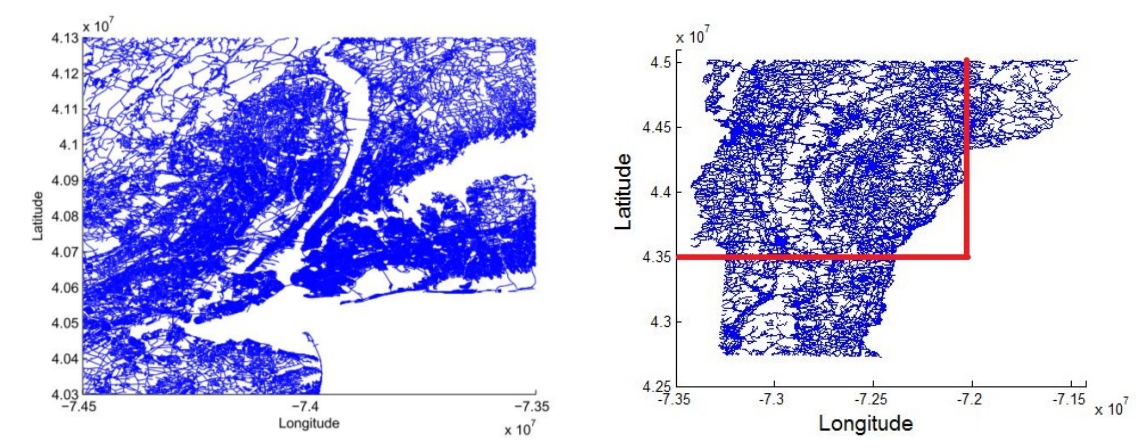
\includegraphics[scale=0.2]{figs/road_maps}
  	\end{figure}
\end{columns} 
\note{This research work employed two different benchmarks, random grids and realistic road maps.  The first experiments were performed on 100 times 100 grids with the start node located in the center of the grid and the target node at different solutions depths from 20 to 100 to the bottom right corner. Horizontal and vertical movements are possible in the grid, with arcs costs randomly generated from one to ten for each of the $q$ criteria. 

We also tested the algorithms in two maps from the 9th DIMACS Shortest Path Challenge, with three metrics, distance and travel time, and the economic cost, calculated as a function of fuel consumption, road types and tolls.}
\end{frame}
%%%%%%%%%%%%%%%%%%%%%%%%%%%%%%%%%%%%%%%%%%%%%%%%%%%%%%%%%%%%%%%%%%%%%%%%%%%%%%%%%%%%%%%%%%%%%%%%%%%%%%%%%
\subsection{Empirical analysis on grids}
\begin{frame}<beamer>[noframenumbering]
\frametitle{Empirical analyses}
	\begin{center}
		\LARGE{\textcolor{ao}{A priori}}
	\end{center}
	\begin{table}
	\centering
	\scalebox{1.5}{
	\begin{tabular}{|lll|}
	\hline \noalign{\smallskip}
	\lexgo & vs & \namoa\\
	\noalign{\smallskip} \hline \noalign{\smallskip}
	\end{tabular}
	}
	\end{table}
\note{}
\end{frame}
 %%%%%%%%%%%%%%%%%%%%%%%%%%%%%%%%%%%%%%%%%%%%%%%%%%%%%%%%%%%%%%%%%%%%%%%%%%%%%%%%%%%%%%%%%%%%%%%%%%%%%%%%%
\begin{frame} 
\frametitle{\lexgo \ vs \namoa}
	\begin{figure}
    	\centering
		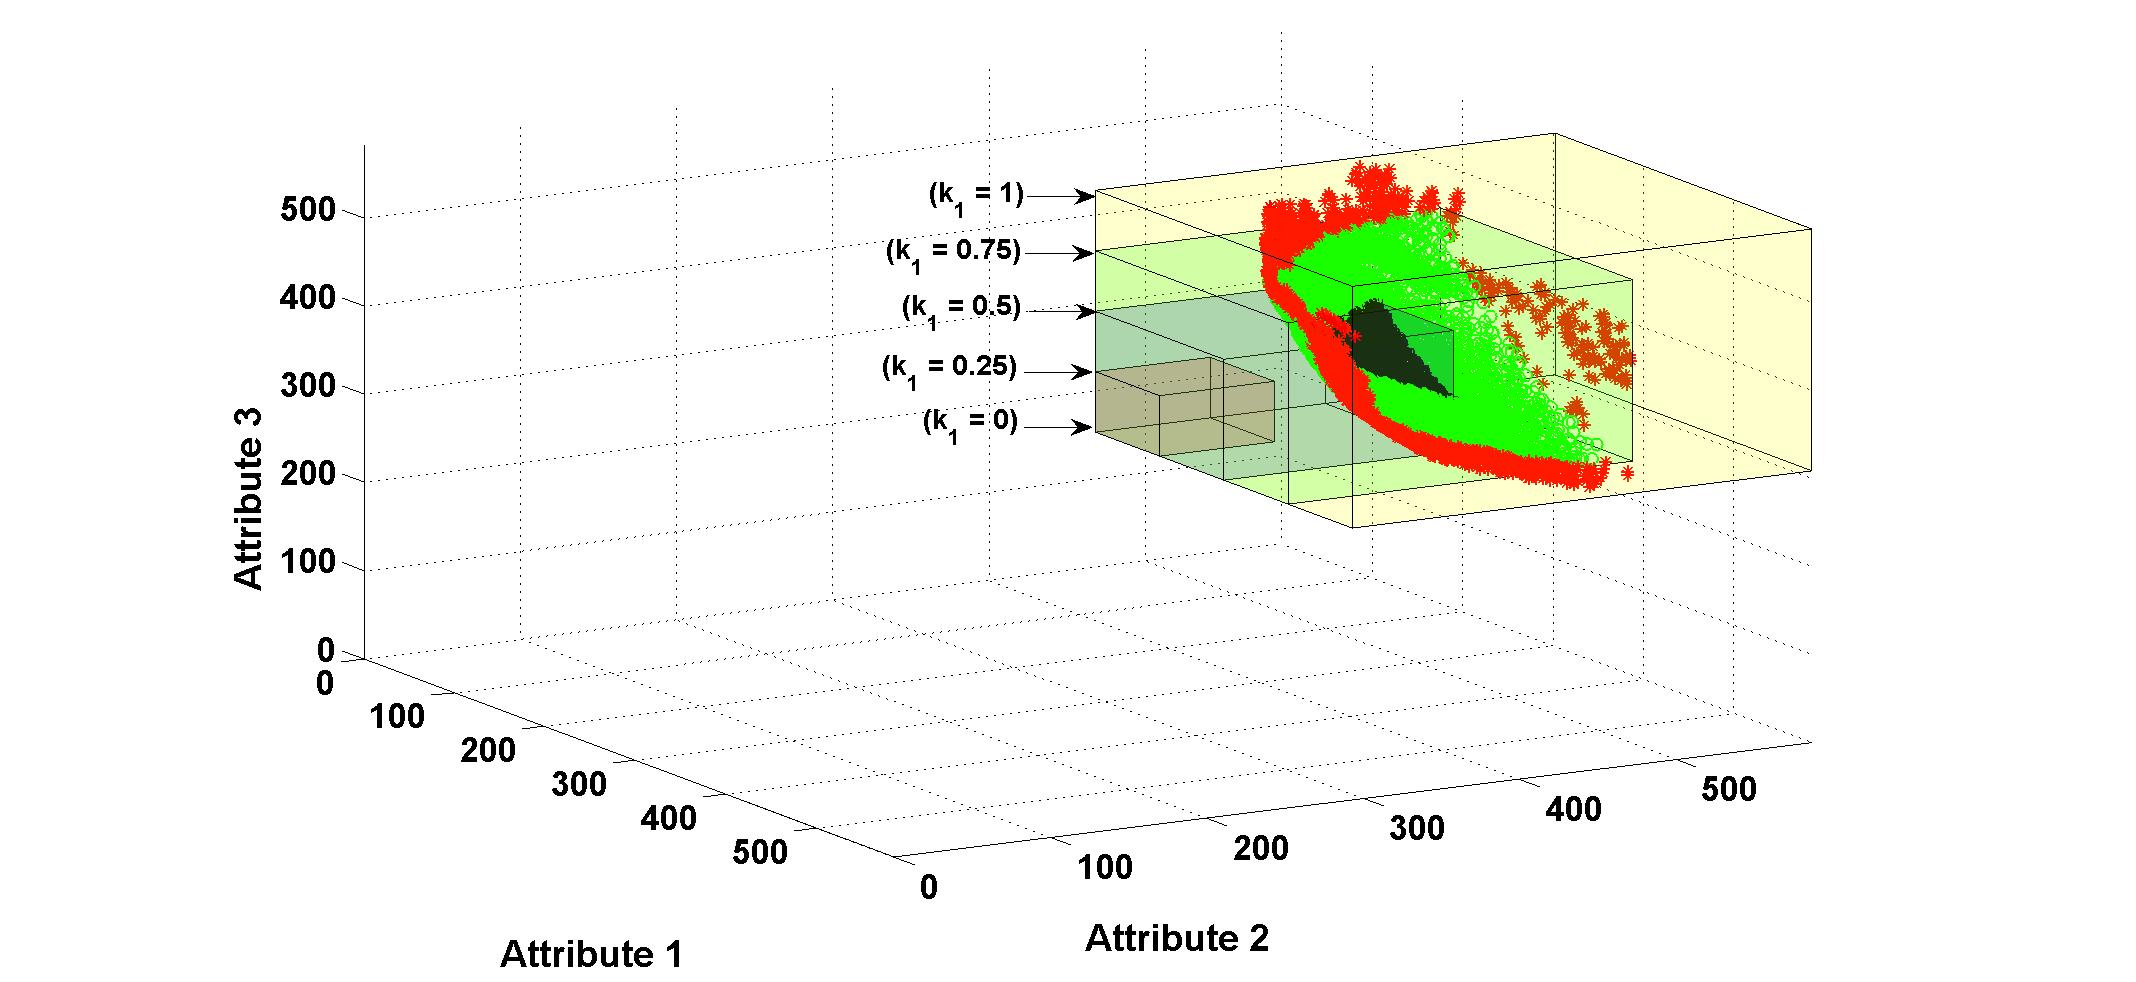
\includegraphics[scale=0.175]{figs/lexgo3d}
	\caption{3D Pareto frontier according to goal satisfiability.}
	\end{figure}
\note{In this figure we see the three dimensional Pareto frontier obtained by \namoa \ for a grid problem. Each of these cubes represent the goals imposed to \lexgo \ in Class I experiments, from the ideal point, located on $k_1$ equals to zero, to the yellow cube that corresponds to goals situated in the nadir point. We can observe that in 0.5 a good percentage of the Pareto frontier would be returned by \lexgo, and in 0.75 the majority of the non-dominated solutions}
\end{frame}
%%%%%%%%%%%%%%%%%%%%%%%%%%%%%%%%%%%%%%%%%%%%%%%%%%%%%%%%%%%%%%%%%%%%%%%%%%%%%%%%%%%%%%%%%%%%%%%%%%%%%%%%%
\begin{frame} 
\frametitle{\lexgo \ vs \namoa}
	\begin{figure}
    	\centering
		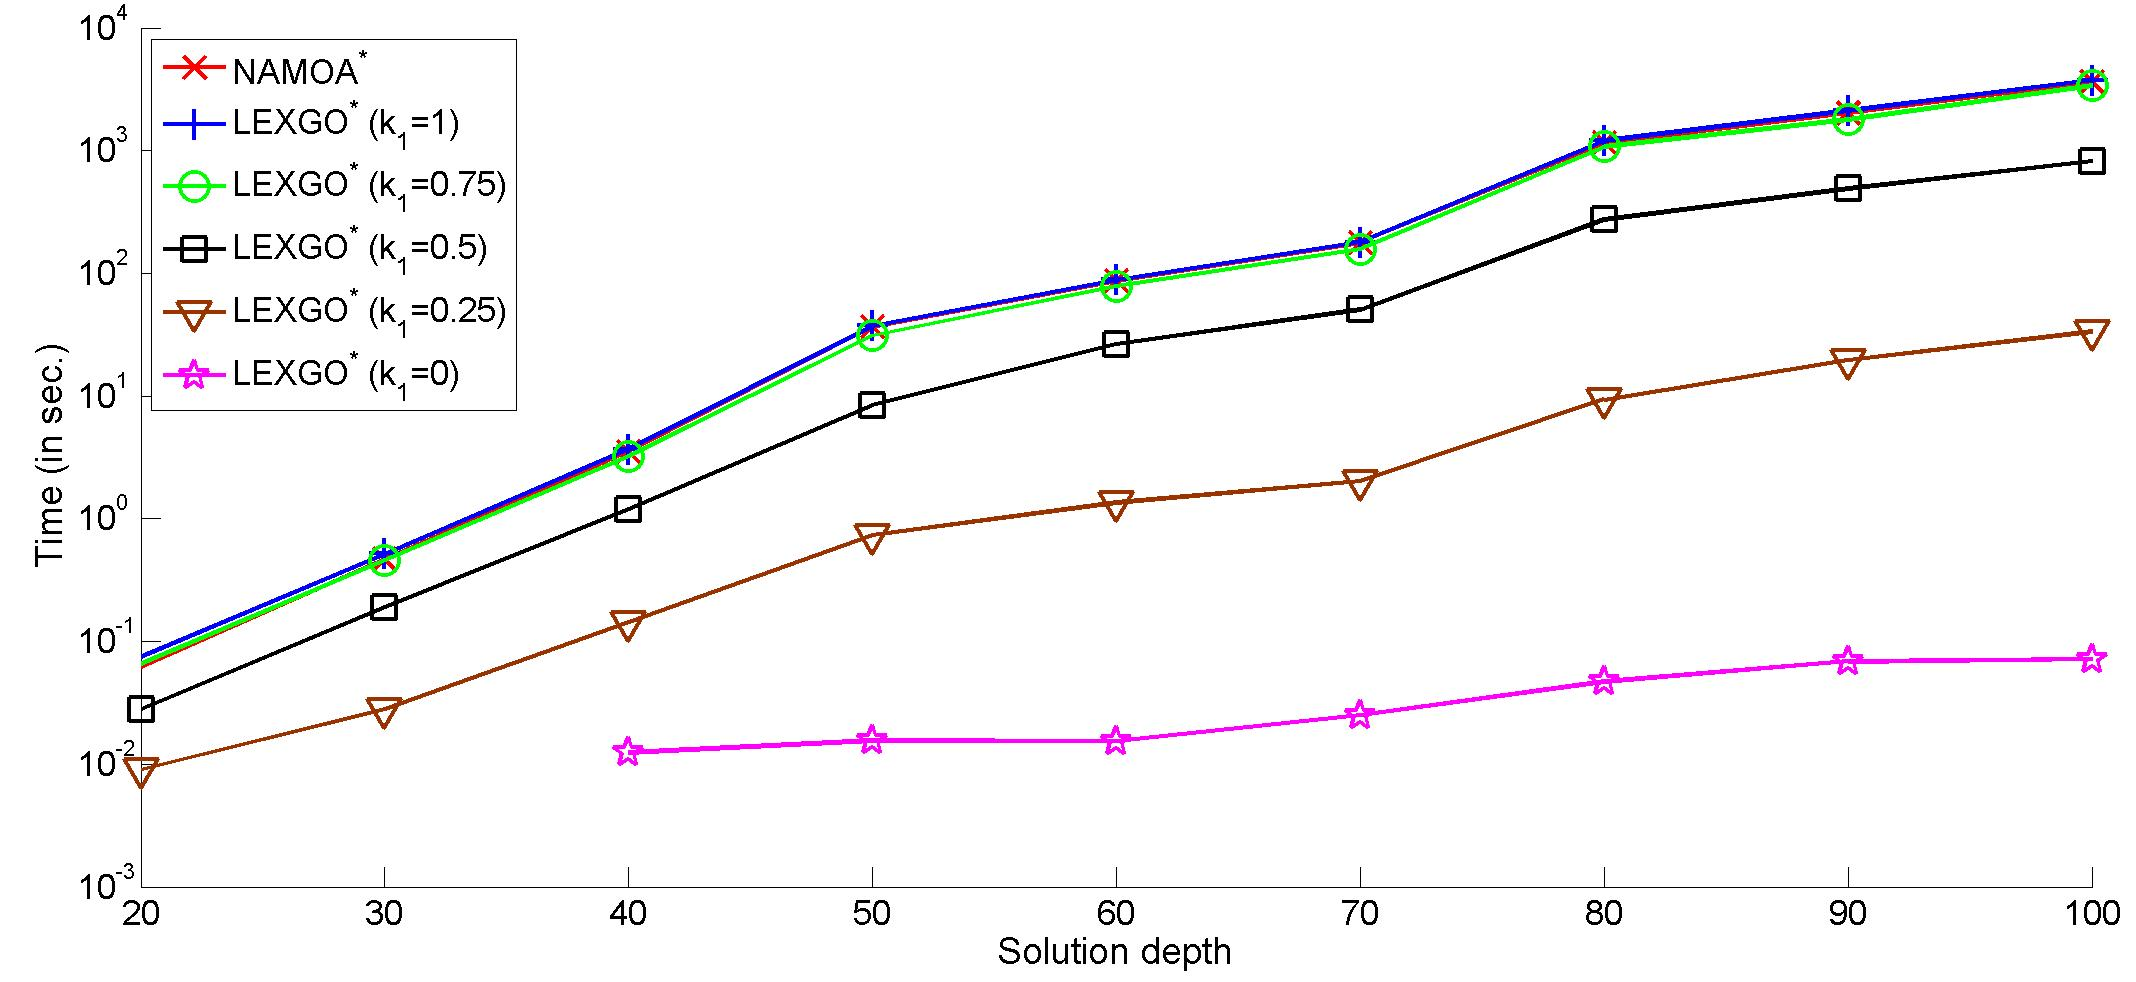
\includegraphics[scale=0.16]{figs/lexgo-exe-time}
		\caption{Runtimes of \namoa \ and \lexgo \ in seconds (logarithmic scale).}
	\end{figure}
\note{}
\end{frame}
%%%%%%%%%%%%%%%%%%%%%%%%%%%%%%%%%%%%%%%%%%%%%%%%%%%%%%%%%%%%%%%%%%%%%%%%%%%%%%%%%%%%%%%%%%%%%%%%%%%%%%%%%
\begin{frame}[t]
\frametitle{\lexgo \ vs \namoa}
	\vspace{5mm}
	\begin{center}
		\begin{table}
		\caption{%
    		Runtimes for $d = 100$ experiments.
     	}%
     	\vspace{2mm}
     		\scalebox{1.2}{
			\begin{tabular}{rrrrrrr}
			\hline \noalign{\smallskip}
			& \multicolumn{5}{c}{\lexgolex} \\
			\noalign{\smallskip} \cline{2-6} \noalign{\smallskip}
			\namoalex & 1 & 0.75 & 0.5 & 0.25 & 0 & \multicolumn{1}{c}{$k_1$} \\
			\noalign{\smallskip} 
			Runtime (s) & \% & \% & \% & \% & \% \\
			\cline{1-6}  \noalign{\smallskip} 
			3,662.9 & 102.7 & \textcolor{ao}{92.3} & \textcolor{ao}{22.3} & \textcolor{ao}{0.9} & \textcolor{ao}{0.001} \\
			\hline
			\end{tabular} 
			}
		\end{table}
	\end{center}
\note{Let's see now the runtime requirements. We also observe here the effectiveness of \lexgo, 5 orders of magnitude faster for k1 equals to 0, two orders of magnitude for k1 in 0.25, 5 times faster for 0.5, slightly faster for 0.75 and with a little overhead when \lexgo \ returns the whole Pareto frontier.
In Class experiments we observe a similar behaviour, \lexgo \ is somewhat around forty to fifty times faster than \namoa \ in these cases (0.75-0.1875, 0.5,0.125)}
\end{frame}
%%%%%%%%%%%%%%%%%%%%%%%%%%%%%%%%%%%%%%%%%%%%%%%%%%%%%%%%%%%%%%%%%%%%%%%%%%%%%%%%%%%%%%%%%%%%%%%%%%%%%%%%%
\begin{frame}<beamer>[noframenumbering]
\frametitle{Empirical analyses}
	\begin{center}
		\LARGE{\textcolor{ao}{A priori}}
	\end{center}
	\begin{table}
	\centering
	\scalebox{1.5}{
	\begin{tabular}{|lll|}
	\hline \noalign{\smallskip}
	\lexgo & vs & \namoa\\
	\noalign{\smallskip} \hline \noalign{\smallskip}
	\lexgodr & vs & \lexgo\\
	\noalign{\smallskip} \hline \noalign{\smallskip}
	\end{tabular}
	}
	\end{table}
\note{}
\end{frame}
%%%%%%%%%%%%%%%%%%%%%%%%%%%%%%%%%%%%%%%%%%%%%%%%%%%%%%%%%%%%%%%%%%%%%%%%%%%%%%%%%%%%%%%%%%%%%%%%%%%%%%%%%
\begin{frame} 
\frametitle{\lexgodr \ vs \lexgo}
	\begin{figure}
    	\centering
		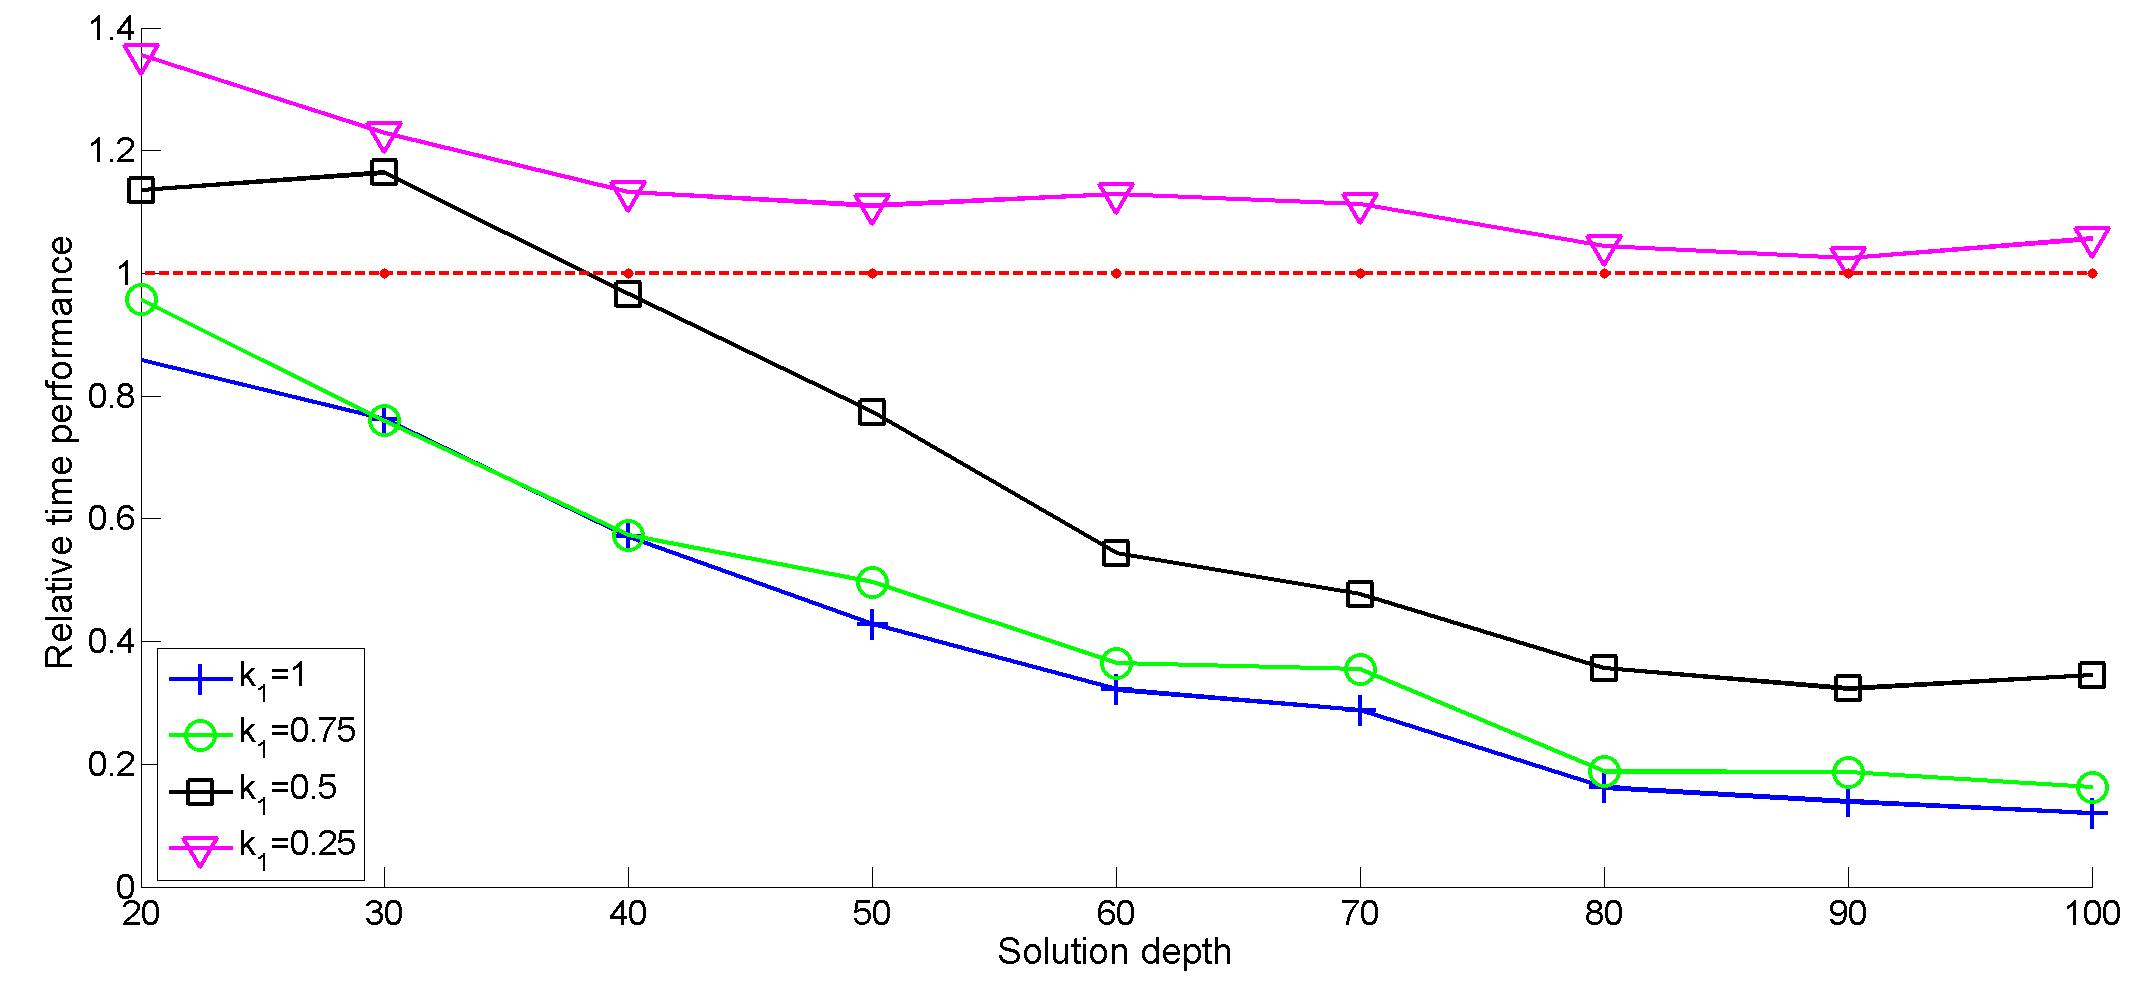
\includegraphics[scale=0.16]{figs/lexgodr-exe-time}
		\caption{Relative runtime performance of \lexgodr \ over \lexgo.}
	\end{figure}
\note{}
\end{frame}
%%%%%%%%%%%%%%%%%%%%%%%%%%%%%%%%%%%%%%%%%%%%%%%%%%%%%%%%%%%%%%%%%%%%%%%%%%%%%%%%%%%%%%%%%%%%%%%%%%%%%%%%%
\begin{frame} 
\frametitle{\lexgodr \ vs \lexgo}
	\begin{table}
	\caption{Runtimes in seconds for $d = 100$ experiments.}
	\vspace{2mm}
	\centering
	\scalebox{1.2}{
	\begin{tabular}{rrrr}
	%\hline \noalign{\smallskip}
	\cline{2-4} \noalign{\smallskip}
	$k_1$ & \lexgolex & \lexgodr & Speedup\\
	\noalign{\smallskip} \hline
	1 & 3,763.78 & 254.40 & \textcolor{ao}{14.81} \\
	0.75 & 3,381.33 & 300.86 & \textcolor{ao}{11.27} \\
	0.5 & 819.28 & 282.49 & \textcolor{ao}{2.90} \\
	0.25 & 33.47 & 35.37 & 0.94 \\
	0 & 0.07 & 0.10 & 0.7\\
	\hline
	\end{tabular}
	}
	\end{table}
\note{Is t-discarding as effective in \lexgo \ as it was in \namoa? To some extent, we see speed ups of 2 to 8 when goals can be satisfied, and obviously nothing we goals can not be satisfied, since t-discarding is not applied then.}
\end{frame}
%%%%%%%%%%%%%%%%%%%%%%%%%%%%%%%%%%%%%%%%%%%%%%%%%%%%%%%%%%%%%%%%%%%%%%%%%%%%%%%%%%%%%%%%%%%%%%%%%%%%%%%%%
\begin{frame}<beamer>[noframenumbering]
\frametitle{Empirical analyses}
	\begin{center}
		\LARGE{\textcolor{ao}{A posteriori}}
	\end{center}
	\begin{table}
	\centering
	\scalebox{1.5}{
	\begin{tabular}{|lll|}
	\hline \noalign{\smallskip}
	\namoadr & vs & \namoa\\
	\noalign{\smallskip} \hline \noalign{\smallskip}
	\end{tabular}
	}
	\end{table}
\note{}
\end{frame}
 %%%%%%%%%%%%%%%%%%%%%%%%%%%%%%%%%%%%%%%%%%%%%%%%%%%%%%%%%%%%%%%%%%%%%%%%%%%%%%%%%%%%%%%%%%%%%%%%%%%%%%%%%
\begin{frame} 
\frametitle{\namoadr \ vs \namoa}
	\begin{figure}
    	\centering
		\includegraphics<1>[scale=0.075]{figs/namoas-exe}
		\caption{Runtimes for \namoalex, \namoalin, and \namoadr \ with $q = \{3, 4, 5\}$}		 
	\end{figure}
\note{We see these improvements here. For three, four or five objectives, the runtimes are greatly reduced and the improvement even grows with problem difficulty. In particular, for three objectives we see here a comparison between the new \namoa \ and both versions of standard \namoa \ with lexicographic and linear selection orders. I'd like to remark that like in other studies, \namoalin \ is somewhat twice as fast as \namoalex, but both are meaningfully slower than \namoadr.}
\end{frame}
%%%%%%%%%%%%%%%%%%%%%%%%%%%%%%%%%%%%%%%%%%%%%%%%%%%%%%%%%%%%%%%%%%%%%%%%%%%%%%%%%%%%%%%%%%%%%%%%%%%%%%%%%
\begin{frame}<beamer>[noframenumbering]
\frametitle{Empirical analyses}
	\begin{center}
		\LARGE{\textcolor{ao}{A posteriori \ vs \ A priori}}
	\end{center}
	\begin{table}
	\centering
	\scalebox{1.5}{
	\begin{tabular}{|lll|}
	\hline \noalign{\smallskip}
	\namoadr & vs & \lexgodr\\
	\noalign{\smallskip} \hline
	\end{tabular}
	}
	\end{table}
\note{}
\end{frame}
%%%%%%%%%%%%%%%%%%%%%%%%%%%%%%%%%%%%%%%%%%%%%%%%%%%%%%%%%%%%%%%%%%%%%%%%%%%%%%%%%%%%%%%%%%%%%%%%%%%%%%%%%
\begin{frame} 
\frametitle{\lexgodr \ vs \namoadr}
	\begin{table}
	\caption{Runtimes of \textcolor{ao}{\lexgodr} \ and \textcolor{red}{\namoadr}.}
	\vspace{2mm}
	\centering
	\scalebox{.9}{
	\begin{tabular}{rrrrrr}
	\hline \noalign{\smallskip}
	 & \multicolumn{5}{c}{\lexgodr} \\
	\noalign{\smallskip} \cline{2-6} \noalign{\smallskip}
	\namoadr & $(k_1=1)$ & $(k_1=0.75)$ & $(k_1=0.5)$ & $(k_1=0.25)$ & $(k_1=0)$ \\
	\noalign{\smallskip} 
	Runtime (s) \\
	\hline  \noalign{\smallskip} 
	100\% & \textcolor{red}{129.7\%} & \textcolor{red}{153.4\%} & \textcolor{red}{144\%} & \textcolor{ao}{18\%} & \textcolor{ao}{0.04\%} \\
	\hline
	\end{tabular}
	}
	\end{table} 
\note{What about the final comparison between the two best alternatives? \namoadr \ is preferable whenever a big amount of non-dominated paths satisfy the goals, and \lexgodr \ when a small number satisfy the goals or they can not be satisfied at all.}
\end{frame}
%%%%%%%%%%%%%%%%%%%%%%%%%%%%%%%%%%%%%%%%%%%%%%%%%%%%%%%%%%%%%%%%%%%%%%%%%%%%%%%%%%%%%%%%%%%%%%%%%%%%%%%%%
\subsection{Empirical analysis on road maps}
\begin{frame}<beamer>[noframenumbering]
\frametitle{Empirical analyses}
	\begin{center}
		\LARGE{\textcolor{ao}{A priori}}
	\end{center}
	\begin{table}
	\centering
	\scalebox{1.5}{
	\begin{tabular}{|lll|}
	\hline \noalign{\smallskip}
	\lexgo & vs & \namoa\\
	\noalign{\smallskip} \hline \noalign{\smallskip}
	\end{tabular}
	}
	\end{table}
\note{}
\end{frame}
 %%%%%%%%%%%%%%%%%%%%%%%%%%%%%%%%%%%%%%%%%%%%%%%%%%%%%%%%%%%%%%%%%%%%%%%%%%%%%%%%%%%%%%%%%%%%%%%%%%%%%%%%%
\begin{frame} 
\frametitle{\lexgo \ vs \namoa}
	\begin{table}
		\caption{Experiments for Vermont State map.}
		\scalebox{1.1}{
		\begin{tabular}{rrrrrrr}
		\hline \noalign{\smallskip}
		 & \multicolumn{5}{c}{\lexgolex} \\
		\noalign{\smallskip} \cline{2-6} \noalign{\smallskip}
		\namoalex & 1 & 0.75 & 0.5 & 0.25 & 0 & \multicolumn{1}{c}{$k_1$}\\
		\noalign{\smallskip} 
		Avg. runtime (s) & \% & \% & \% & \% & \% & \\
		\cline{1-6} \noalign{\smallskip} 
		5,048.47 & 100.39 & \textcolor{ao}{74.67} & \textcolor{ao}{29.06} & \textcolor{ao}{3.51} & \textcolor{ao}{0.01} \\
		\hline
		\end{tabular}
		}
	\end{table}
\note{The runtime requirements are also equivalent to the relative performance shown in grids, with greater advantage of \lexgo \ when goals are more restrictive and less non-dominated paths satisfy the goals.}
\end{frame}
%%%%%%%%%%%%%%%%%%%%%%%%%%%%%%%%%%%%%%%%%%%%%%%%%%%%%%%%%%%%%%%%%%%%%%%%%%%%%%%%%%%%%%%%%%%%%%%%%%%%%%%%%
\begin{frame}<beamer>[noframenumbering]
\frametitle{Empirical analyses}
	\begin{center}
		\LARGE{\textcolor{ao}{A priori}}
	\end{center}
	\begin{table}
	\centering
	\scalebox{1.5}{
	\begin{tabular}{|lll|}
	\hline \noalign{\smallskip}
	\lexgo & vs & \namoa\\
	\noalign{\smallskip} \hline \noalign{\smallskip}
	\lexgodr & vs & \lexgo\\
	\noalign{\smallskip} \hline \noalign{\smallskip}
	\end{tabular}
	}
	\end{table}
\note{}
\end{frame}
%%%%%%%%%%%%%%%%%%%%%%%%%%%%%%%%%%%%%%%%%%%%%%%%%%%%%%%%%%%%%%%%%%%%%%%%%%%%%%%%%%%%%%%%%%%%%%%%%%%%%%%%%
\begin{frame} 
\frametitle{\lexgodr \ vs \lexgo}
	\begin{table}
	\caption{Runtimes in seconds for Vermont State map.}
	\vspace{2mm}
	\centering
	\begin{tabular}{rrrrrrrr}
	\hline \noalign{\smallskip}
 	& 1 & 0.75 & 0.5 & 0.25 & 0 & \multicolumn{1}{c}{$k_1$}\\
	\noalign{\smallskip} 
	\cline{2-6} \noalign{\smallskip} 
	\lexgolex & 5,068.00 & 3,769.51 & 1,467.00 & 177.33 & 0.03 \\
	%\lexgolin & 4,716.90 & 3,497.26 & 1,287.37 & 205.39 & 0.03 \\
	\textcolor{red}{\lexgodr} & \textcolor{ao}{94.90} &	\textcolor{ao}{83.59} & \textcolor{ao}{57.38} & \textcolor{ao}{157.02} & \textcolor{ao}{0.03} \\
	\hline
	\end{tabular}
	\end{table}
\note{The same impressive improvements can be seen when we apply t-discarding to \lexgo \ and goals can be satisfied, with 0.5, 0.75 and 1.}
\end{frame}
%%%%%%%%%%%%%%%%%%%%%%%%%%%%%%%%%%%%%%%%%%%%%%%%%%%%%%%%%%%%%%%%%%%%%%%%%%%%%%%%%%%%%%%%%%%%%%%%%%%%%%%%%
\begin{frame}<beamer>[noframenumbering]
\frametitle{Empirical analyses}
	\begin{center}
		\LARGE{\textcolor{ao}{A posteriori}}
	\end{center}
	\begin{table}
	\centering
	\scalebox{1.5}{
	\begin{tabular}{|lll|}
	\hline \noalign{\smallskip}
	\namoadr & vs & \namoa\\
	\noalign{\smallskip} \hline \noalign{\smallskip}
	\end{tabular}
	}
	\end{table}
\note{}
\end{frame}
%%%%%%%%%%%%%%%%%%%%%%%%%%%%%%%%%%%%%%%%%%%%%%%%%%%%%%%%%%%%%%%%%%%%%%%%%%%%%%%%%%%%%%%%%%%%%%%%%%%%%%%%%
\begin{frame} 
\frametitle{\namoadr \ vs \namoa}
	\begin{figure}
    	\centering
		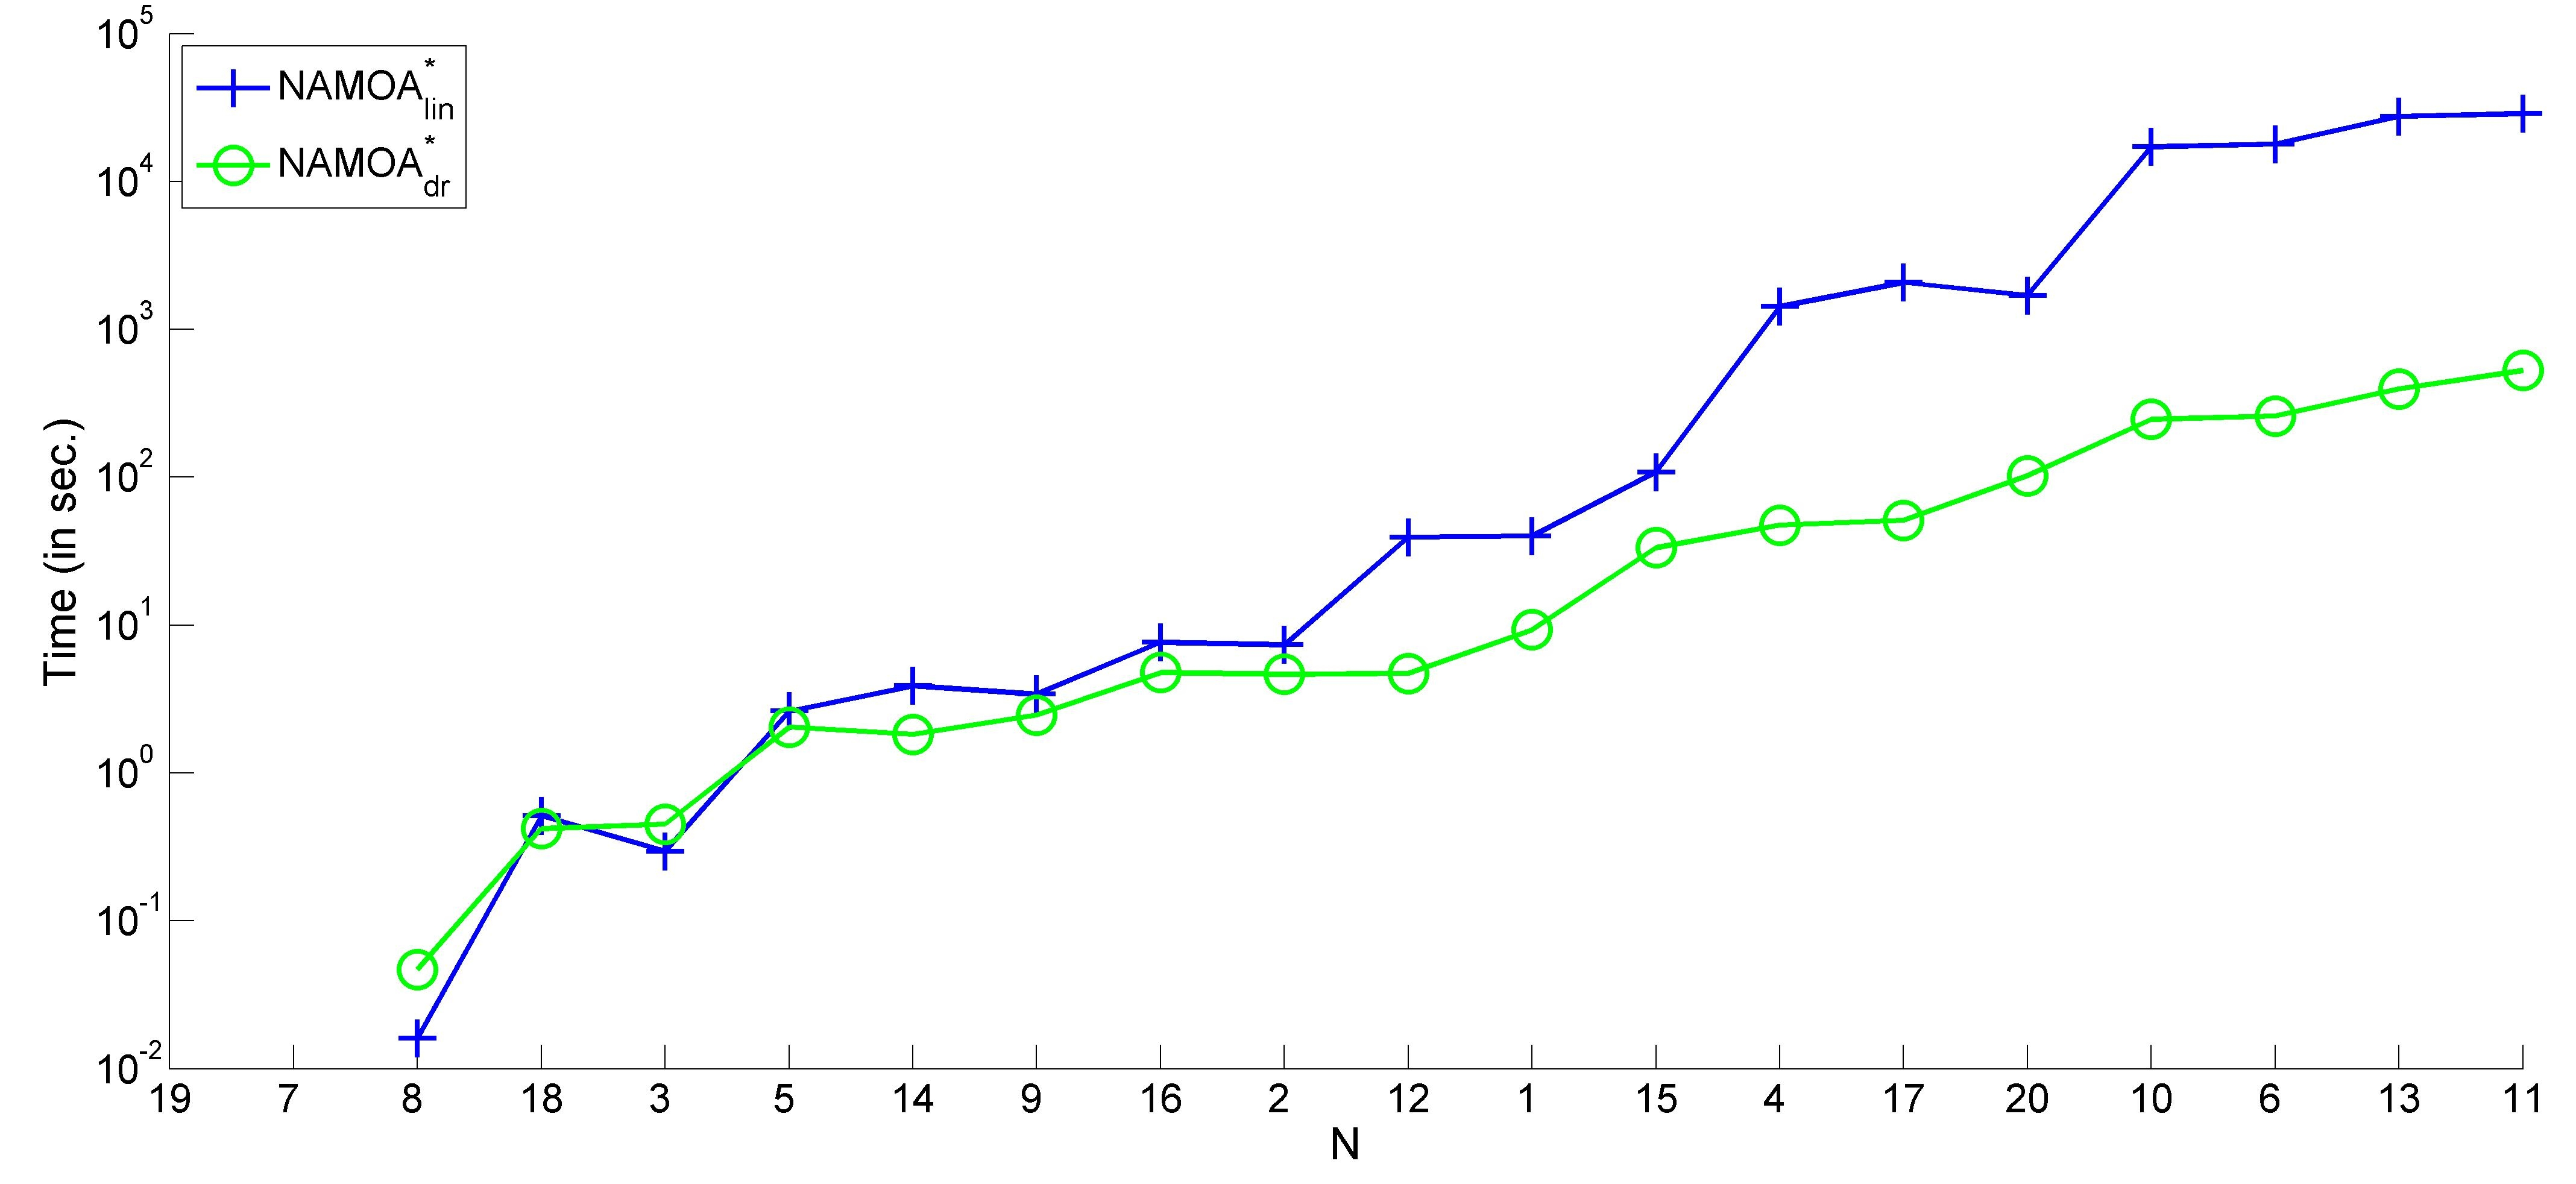
\includegraphics[scale=0.1]{figs/namoadr-roads-exe}
	\caption{Runtimes of \namoalin \ and \namoadr \ for Vermont map problems.}
	\end{figure}
\end{frame}
%%%%%%%%%%%%%%%%%%%%%%%%%%%%%%%%%%%%%%%%%%%%%%%%%%%%%%%%%%%%%%%%%%%%%%%%%%%%%%%%%%%%%%%%%%%%%%%%%%%%%%%%%
\begin{frame}<beamer:0>
\frametitle{\namoadr \ vs \namoa}
	\begin{table}
	\caption{Experimental summary for Vermont State map.}
		\vspace{2mm}
		\scalebox{1.2}{
		\begin{tabular}{ccccccc}
		\noalign{\smallskip} \hline \noalign{\smallskip}
		Map & $t_{\text{NAMOA}^* \text{lin}}$ & $t_{\text{NAMOA}^* \text{dr}}$ & \% \\
		\noalign{\smallskip} \hline \noalign{\smallskip}
		VT$_{cut}$ & 4,838.4 s. & \textcolor{ao}{84.6 s.} & \textcolor{red}{1.74} \\
		\noalign{\smallskip} \hline
		\end{tabular} 
		}
	\end{table}
\note{We see them first in this graphic, whenever the query becomes more time consuming, the advantage of the t-discarding version also grows. Moreover, in this table, the average runtime for \namoalin, the fastest previous version of \namoa, was 4 thousand and 8 hundred seconds, about 1 hour and 20 minutes, while \namoadr \ average runtime is less than one minute and a half.}
\end{frame}
%%%%%%%%%%%%%%%%%%%%%%%%%%%%%%%%%%%%%%%%%%%%%%%%%%%%%%%%%%%%%%%%%%%%%%%%%%%%%%%%%%%%%%%%%%%%%%%%%%%%%%%%%
\begin{frame}<beamer>[noframenumbering]
\frametitle{Empirical analyses}
	\begin{center}
		\LARGE{\textcolor{ao}{A posteriori \ vs \ A priori}}
	\end{center}
	\begin{table}
	\centering
	\scalebox{1.5}{
	\begin{tabular}{|lll|}
	\hline \noalign{\smallskip}
	\namoadr & vs & \lexgodr\\
	\noalign{\smallskip} \hline
	\end{tabular}
	}
	\end{table}
\note{}
\end{frame}
%%%%%%%%%%%%%%%%%%%%%%%%%%%%%%%%%%%%%%%%%%%%%%%%%%%%%%%%%%%%%%%%%%%%%%%%%%%%%%%%%%%%%%%%%%%%%%%%%%%%%%%%%
\begin{frame} 
\frametitle{\lexgodr \ vs \namoadr}
	\begin{table}
	\caption{Runtimes in seconds of \textcolor{ao}{\lexgodr} \ and \textcolor{red}{\namoadr} in Vermont State map problems.}
	\vspace{2mm}
	\centering
	\begin{tabular}{rrrrrrr}
	\hline \noalign{\smallskip}
	 & \multicolumn{5}{c}{\lexgodr} \\
	\noalign{\smallskip} \cline{2-6} \noalign{\smallskip}
	\namoadr & 1 & 0.75 & 0.5 & 0.25 & 0 & \multicolumn{1}{c}{$k_1$}\\
	\noalign{\smallskip} 
	\cline{1-6} \noalign{\smallskip} 
	84.66 & \textcolor{red}{94.89} & \textcolor{ao}{83.59} & \textcolor{ao}{57.38} & \textcolor{red}{157.02} & \textcolor{ao}{0.03} \\
	\hline
	\end{tabular}
	\end{table} 
\note{and the final comparison between the two best algorithmic alternatives gives us better results for \namoadr \ than we achieved in random grids, and the particular case here with 0.25. Even though the number of labels expanded is greatly reduced, t-discarding cannot be applied in that case, and therefore, \lexgodr \ runtime is almost two times slower.}
\end{frame}
%%%%%%%%%%%%%%%%%%%%%%%%%%%%%%%%%%%%%%%%%%%%%%%%%%%%%%%%%%%%%%%%%%%%%%%%%%%%%%%%%%%%%%%%%%%%%%%%%%%%%%%%%
\begin{frame} 
\frametitle{Empirical analyses}
\begin{center}
\Huge Why do the new algorithms have \textcolor{ao}{such a runtime performance}?
\end{center}
\end{frame}
%%%%%%%%%%%%%%%%%%%%%%%%%%%%%%%%%%%%%%%%%%%%%%%%%%%%%%%%%%%%%%%%%%%%%%%%%%%%%%%%%%%%%%%%%%%%%%%%%%%%%%%%%
\begin{frame} 
\frametitle{\lexgo \ vs \namoa}
	\begin{figure}
    	\centering
		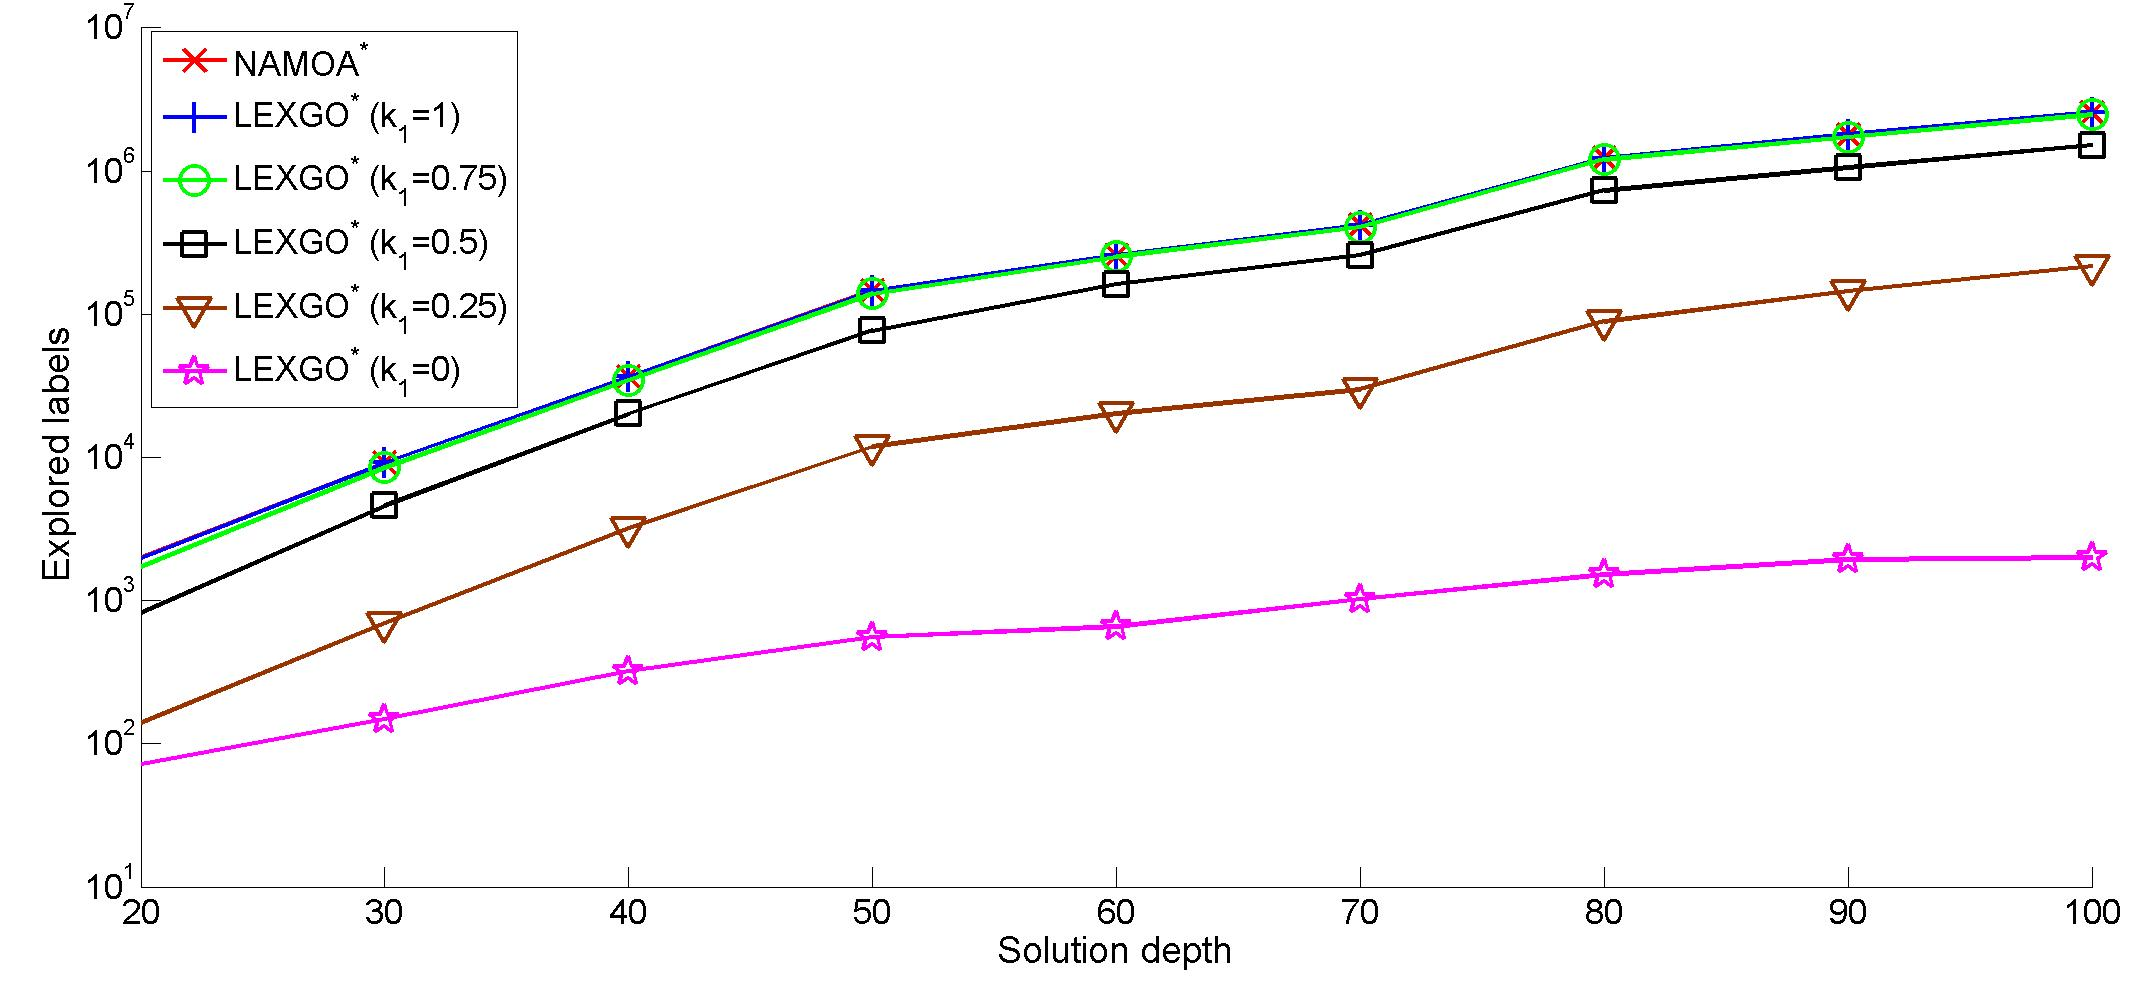
\includegraphics[scale=0.16]{figs/lexgo-labels}
		\caption{Explored labels by \namoa \ and \lexgo \ in grids.}
	\end{figure}
\note{We can observe a reduction of expanded labels of several orders of magnitude for \lexgo \ when k1 is equal to 0 or 0.25. The more restrictive the goals are the greater is that reduction. We can also observe that in the second class of experiments when the second level gets more restrictive.}
\end{frame}
%%%%%%%%%%%%%%%%%%%%%%%%%%%%%%%%%%%%%%%%%%%%%%%%%%%%%%%%%%%%%%%%%%%%%%%%%%%%%%%%%%%%%%%%%%%%%%%%%%%%%%%%%
\begin{frame} 
\frametitle{Deviation-based pruning}
	\begin{figure}
    	\centering
		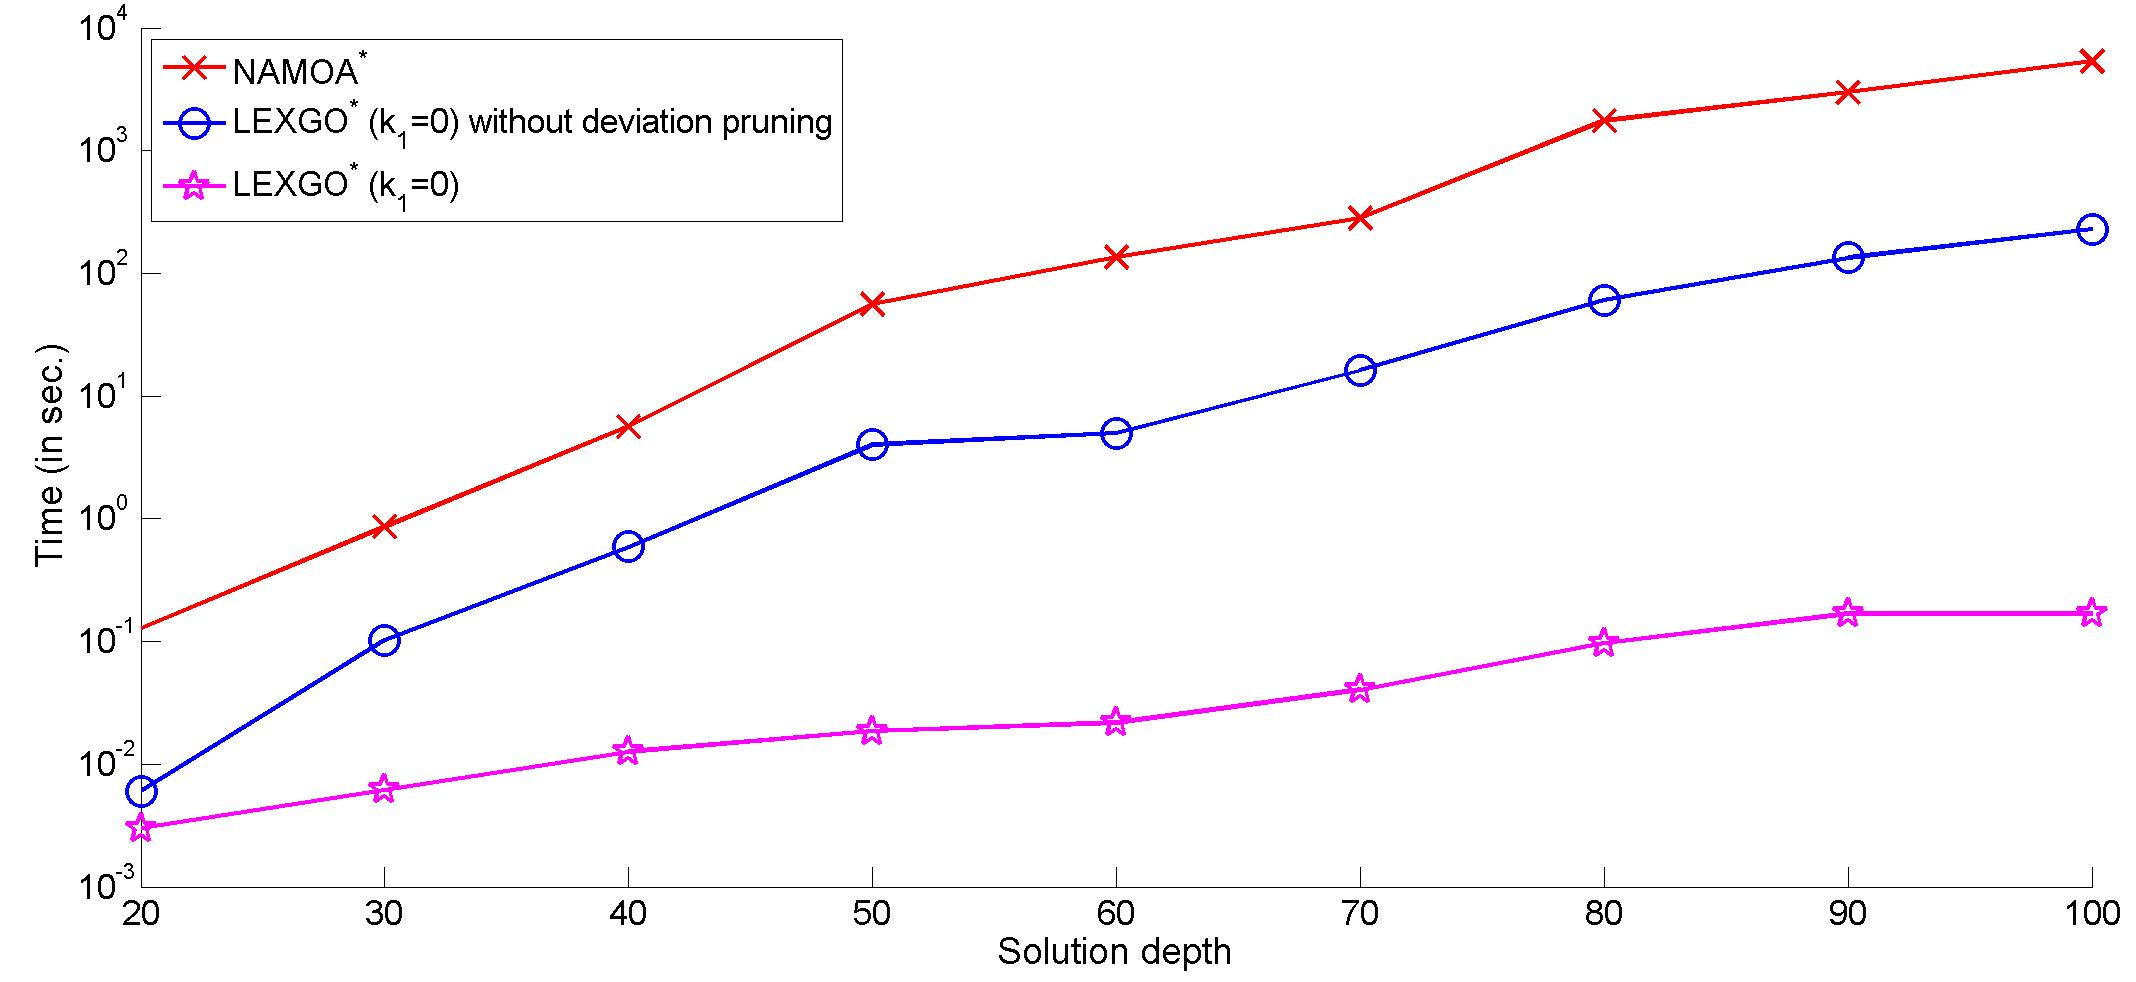
\includegraphics[scale=0.16]{figs/lexgo-dev-pruning}
	\caption{Impact of deviation pruning in $k_1 = 0$ experiments.}
	\end{figure}
\note{In this graphic we see the runtimes of \namoa \ and \lexgo \ with goals in the ideal point with and without using the deviation-based pruning. For the most difficult problems, the runtimes without this rule vary from minutes to tenths of a second.}
\end{frame}
%%%%%%%%%%%%%%%%%%%%%%%%%%%%%%%%%%%%%%%%%%%%%%%%%%%%%%%%%%%%%%%%%%%%%%%%%%%%%%%%%%%%%%%%%%%%%%%%%%%%%%%%%
\begin{frame} 
\frametitle{\namoadr \ vs \namoa}
	\begin{table}
	\caption{Set sizes for Vermont State map.}
		\vspace{2mm}
		\scalebox{1.2}{
		\begin{tabular}{ccc}
		\hline \noalign{\smallskip}
		Map & $(\frac{\sum T(G_{cl})}{\sum G_{cl}})$\% & $(\frac{\sum T(C^*)}{\sum C^*})$\% \\
		\noalign{\smallskip} \hline \noalign{\smallskip} 
VT$_{cut}$ & \textcolor{red}{3.43} & \textcolor{red}{2.45} \\
		\noalign{\smallskip} \hline
		\end{tabular} 
		}
	\end{table}
\note{The relative size of the truncated sets is also reduced to 2 to 3\% of the size of the standard sets Gcl and COSTS.}
\end{frame}
%%%%%%%%%%%%%%%%%%%%%%%%%%%%%%%%%%%%%%%%%%%%%%%%%%%%%%%%%%%%%%%%%%%%%%%%%%%%%%%%%%%%%%%%%%%%%%%%%%%%%%%%%
\begin{frame}
\frametitle{\namoadr \ vs \namoa}
	\begin{figure}
    	\centering
		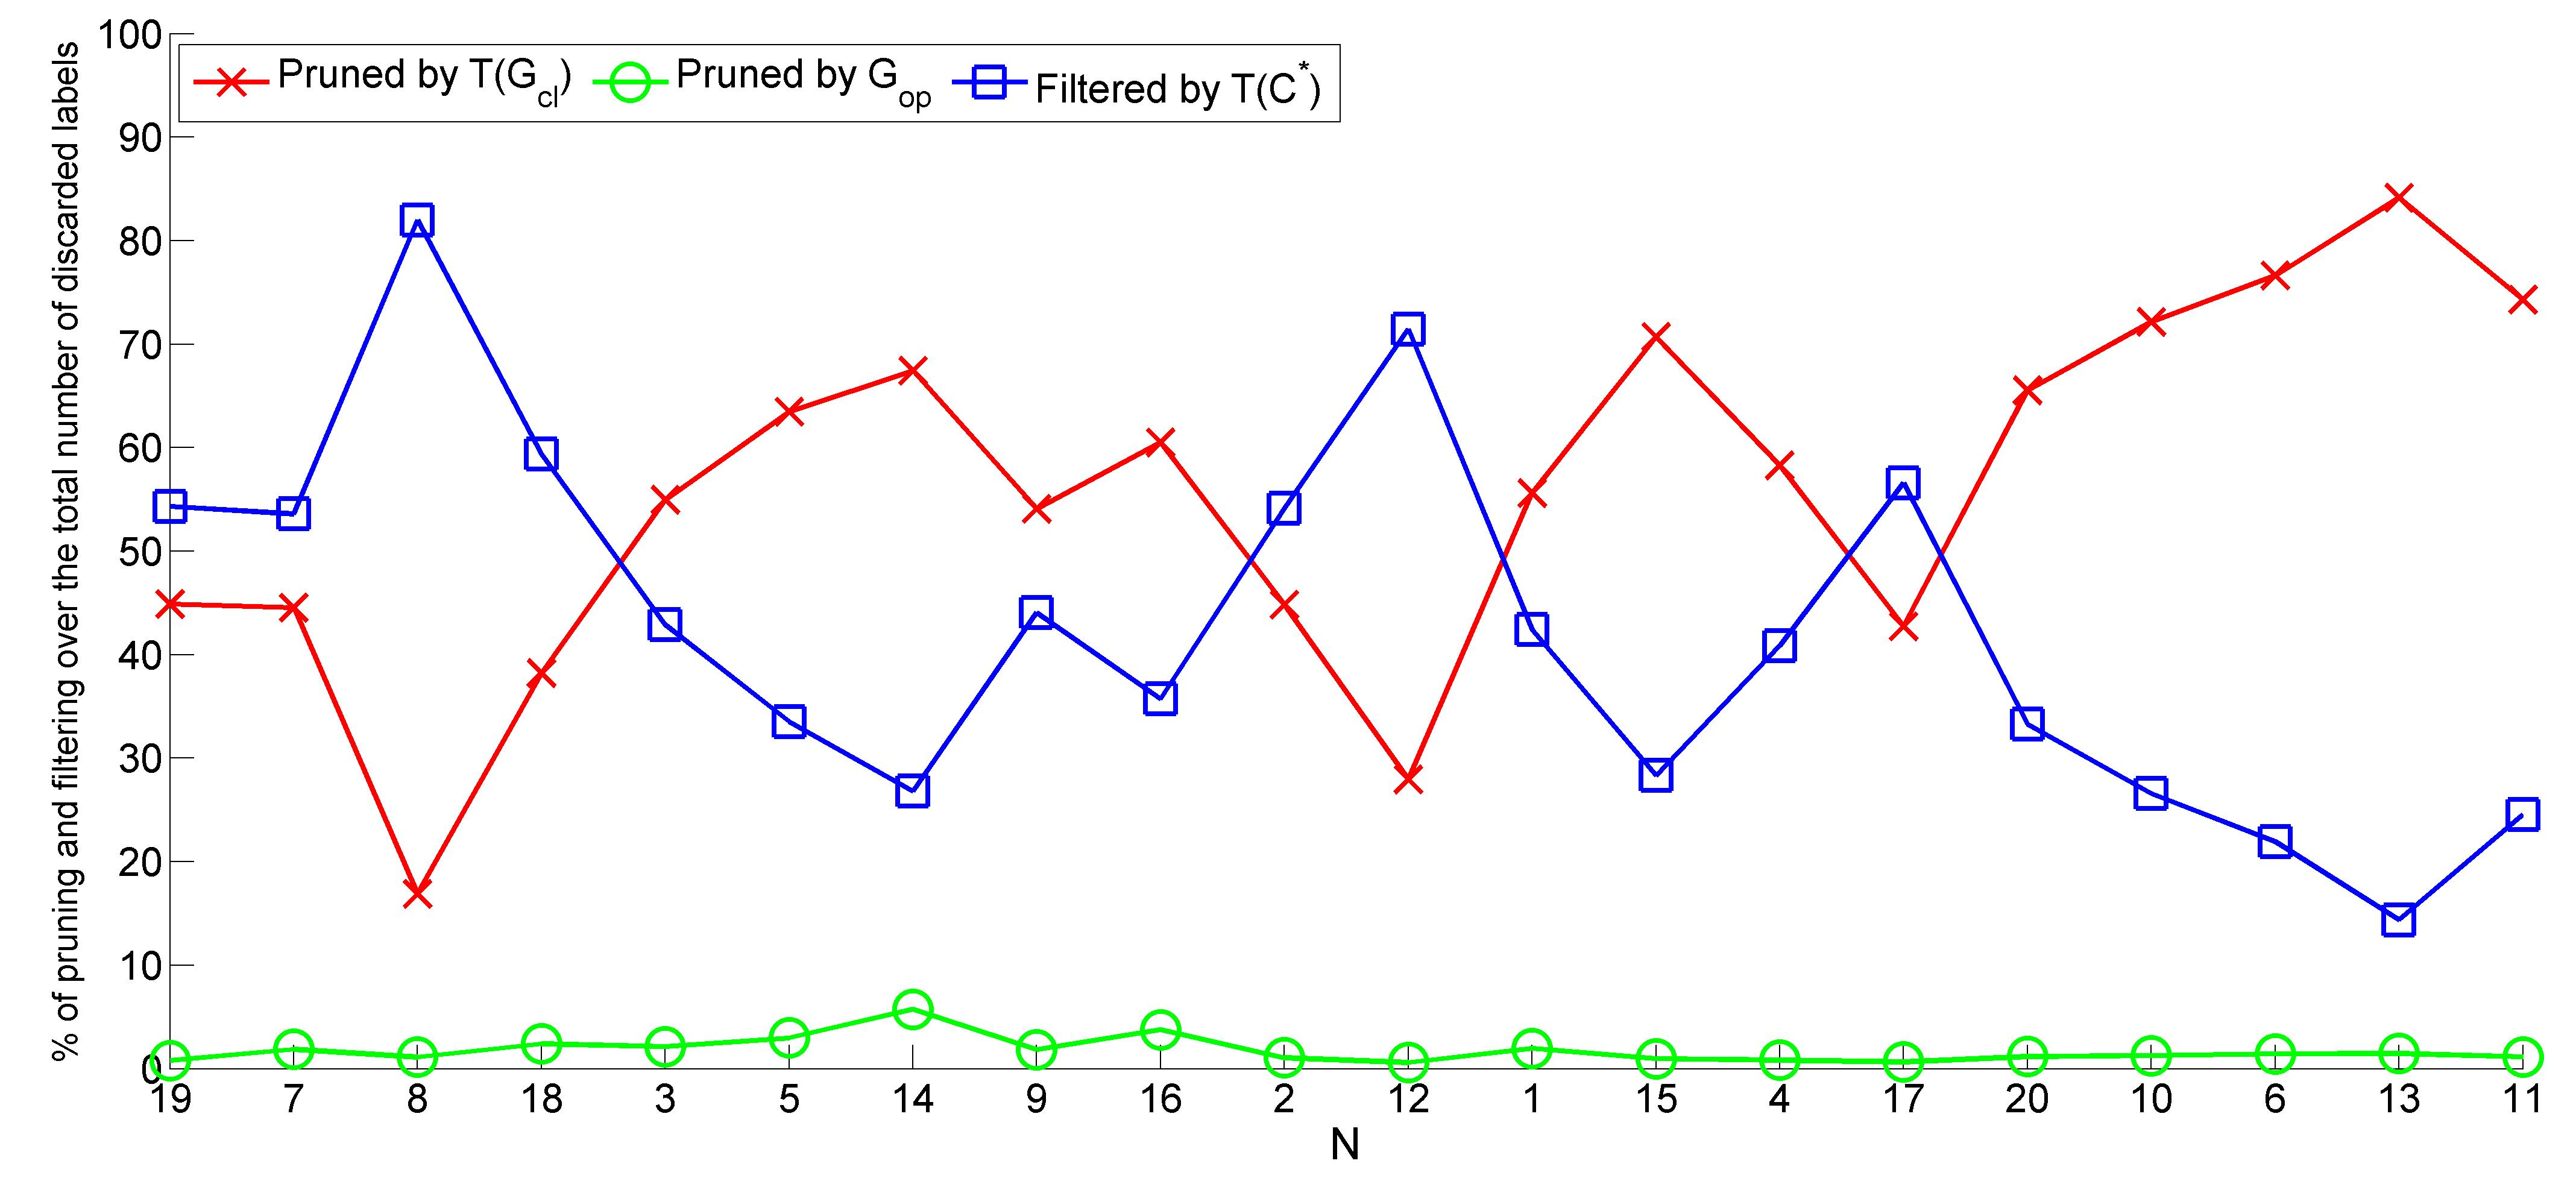
\includegraphics[scale=0.08]{figs/pruned-filtered-vermont}
	\caption{Discarded labels in Vermont problems.}
	\end{figure}
\note{The percentage of labels pruned by Gop is even smaller for road maps, so that, we can expect even bigger runtime improvements in this domain.}
\end{frame}
%%%%%%%%%%%%%%%%%%%%%%%%%%%%%%%%%%%%%%%%%%%%%%%%%%%%%%%%%%%%%%%%%%%%%%%%%%%%%%%%%%%%%%%%%%%%%%%%%%%%%%%%%
\begin{frame} 
\frametitle{New York experiments}
	\LARGE{Now, we can even solve \textcolor{red}{more} problems!}
	\vspace{5mm}
	\begin{table}
	\centering
	\scalebox{1}{
	\begin{tabular}{crr}
	\hline \noalign{\smallskip}
	Problem \# & \namoadr & \namoalin \\
	\noalign{\smallskip} \hline \noalign{\smallskip}
	\#11 & \textcolor{red}{30 min.} & 31 hours \\
	\noalign{\smallskip} \hline \noalign{\smallskip}
	\#6 & \textcolor{red}{3 hours} & 25 days \\
	\noalign{\smallskip} \hline
	\end{tabular}
	}
	\end{table}
\note{As an example, we are going to show now the runtimes of \namoadr \ and \namoalin \ sorted by increasing difficulty. The easiest problem of New York was solved by both algorithms really fast. The second problem was solved by \namoadr \ twice as fast as \namoalin. The third problem, number 16, was solved around 6 times faster. The fourth problem was solved by \namoadr \ in two minutes and half and more than an hour by the standard version of \namoa. The fifth problem by difficulty was solved by \namoadr \ in less than half an hour, and it tood 31 hours to be solved by \namoalin, in other words, a speed up of more than sixty. Problem six, was solved in about three hours by \namoadr \ and the impressive amount of 25 days by \namoalin. We can easily see where this is going if we wanted to keep solving problems with \namoalin.}
\end{frame}
%%%%%%%%%%%%%%%%%%%%%%%%%%%%%%%%%%%%%%%%%%%%%%%%%%%%%%%%%%%%%%%%%%%%%%%%%%%%%%%%%%%%%%%%%%%%%%%%%%%%%%%%%
